% \documentclass{article}
% \usepackage{beamerarticle}
\documentclass{beamer}
% Beamer theme settings
\usetheme{Madrid}
\usecolortheme{default}
\usepackage{amsmath}
\usepackage{tikz}
\usepackage{mathtools}
\usepackage{hyperref}
\usetikzlibrary{intersections}
\usepackage{graphicx}
\usepackage{svg}
\usepackage{xcolor}



% Define commands for vectors
\newcommand{\va}{\mathbf{a}}
\newcommand{\vb}{\mathbf{b}}
\newcommand{\vc}{\mathbf{c}}
\newcommand{\vd}{\mathbf{d}}
\newcommand{\ve}{\mathbf{e}}
\newcommand{\vv}{\mathbf{v}}
\newcommand{\vu}{\mathbf{u}}
\newcommand{\vw}{\mathbf{w}}
\newcommand{\vx}{\mathbf{x}}
\newcommand{\vy}{\mathbf{y}}
\newcommand{\vz}{\mathbf{z}}
\newcommand{\N}{\mathbb{N}}
\newcommand{\Z}{\mathbb{Z}}
\newcommand{\R}{\mathbb{R}}
\newcommand{\Q}{\mathbb{Q}}
\newcommand{\rank}{\text{rank}}







% Title page

\title[Lecture 6]{Taylor Series, Integral}
\author[Aprikyan, Tarkhanyan]{Hayk Aprikyan, Hayk Tarkhanyan}
\institute[ACA]{Armenian Code Academy}
\date{November 14, 2024}


\begin{document}

\begin{frame}
  \titlepage
\end{frame}


% slide 1: convex
\begin{frame}{Convex and Concave Functions}
    We know that the sign of the derivative tells us whether a function is increasing or decreasing; for example, when \(f'(x) > 0\), \(f(x)\) is increasing. \pause However, a function can increase like this
    \[
 \includesvg[ width=0.31\textwidth, keepaspectratio]{conv} \pause \qquad\text{or like this} \qquad \includesvg[ width=0.31\textwidth, keepaspectratio]{conc}
\]

\pause 
How can you determine which way it is?

\end{frame}



% slide 1: convex
\begin{frame}{Convex and Concave Functions}
    \begin{block}{Definition}
        A function $f: \mathbb{R} \to \mathbb{R}$ is \textbf{convex} on an interval $I$ if, for any $x_1, x_2$ in $I$ and any $0 \le \lambda \le 1$:
        \[
        f(\textcolor{red}{\lambda} x_1 + (\textcolor{blue}{1-\lambda})x_2) \leq \textcolor{red}{\lambda} f(x_1) + (\textcolor{blue}{1-\lambda}) f(x_2)
        \] \pause
        and \textbf{concave} if
        \[
        f(\textcolor{red}{\lambda} x_1 + (\textcolor{blue}{1-\lambda})x_2) \ge \textcolor{red}{\lambda} f(x_1) + (\textcolor{blue}{1-\lambda}) f(x_2)
        \]
    \end{block}
    Visually this means that if you connect two points on the graph of $f(x)$ with a straight line, if the line is above the curve, $f(x)$ is convex; if it's under the curve, $f(x)$ is concave.
    \linebreak
    
    \\



- \color{blue} \href{https://www.geogebra.org/classic/pn5xhfnr}{Play with $\lambda$ on the graph of a convex function!}

  \end{frame}



% slide 1: convex
\begin{frame}{Convex and Concave Functions}
        \begin{center}

    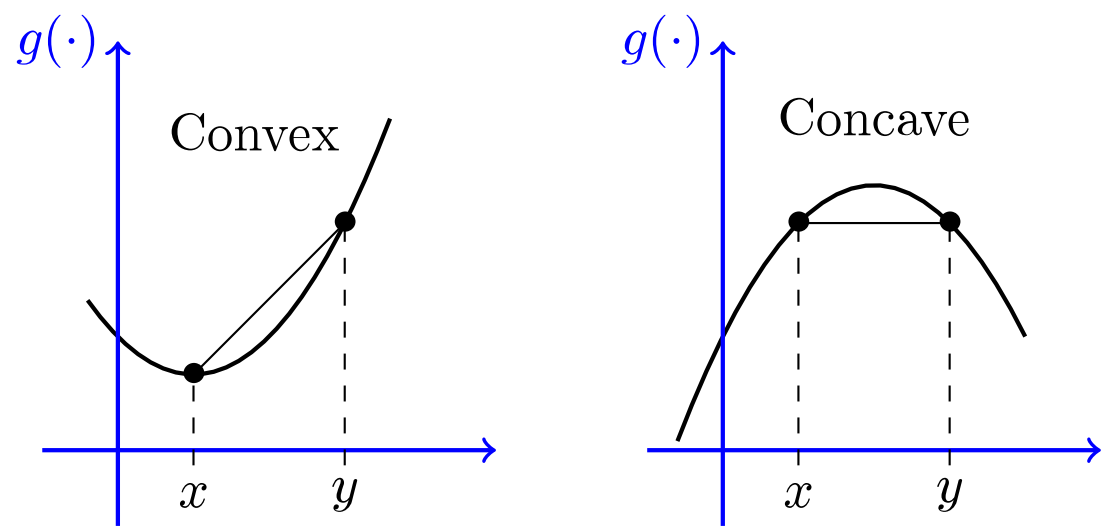
\includegraphics[width=0.9\textwidth, height=\textheight, keepaspectratio]{cxcv.png}
  \end{center}
\pause
    \begin{block}{Theorem}
        If $f(x)$ is a twice-differentiable function (i.e. there exists $f''(x)$), then it is:
        \begin{itemize}
            \item Convex if and only if $f''(x) \ge 0,$
            \item Concave if and only if $f''(x) \le 0.$
        \end{itemize}
    \end{block}
\end{frame}



% slide 1: convex
\begin{frame}{Convex and Concave Functions}
    
    \begin{exampleblock}{Examples}
        \begin{enumerate}
            \item $f(x) = x^2$ is convex on $(-\infty, \infty)$.
            \\ $f''(x) = 2 > 0$
            \item $f(x) = -x^2$ is concave on $(-\infty, \infty)$.
            \\ $f''(x) = -2< 0$
            \item $f(x) = x$ is both convex and concave on $(-\infty, \infty)$.
            \\ $f''(x) = 0 $
            \item $f(x) = \sin x$ is concave on \pause $(0, \pi)$, \pause convex on $(\pi, 2\pi)$. \\\textit{(The endpoints of the intervals can be included freely)}
            \\ $f''(x) = (\cos x)' = -\sin x$
        \end{enumerate}
    \end{exampleblock}
\end{frame}


% slide 2: taylor
\begin{frame}{Taylor Series}
    For a fairly big number of functions, their derivatives tell too much about them. So can they be used to approximate the values of a given function? 
    
    \pause Suppose we have a function $f(x)$ and we construct another function $g(x)$ which, at some point $x_0$:\pause
    \begin{itemize}[<+->]
        \item Has the same value as $f$
        \item Has the same rate of change as $f$
        \item Has the same rate of the rate of change as $f$
        \item \dots 
    \end{itemize}
    \pause Or, equivalently, $g(x_0) = f(x_0)$, $g'(x_0) = f'(x_0)$, $g''(x_0) = f''(x_0)$, \dots,  $g^{(n)}(x_0) = f^{(n)}(x_0)$, \dots.

    \pause Then we could use $g(x)$ to approximate $f(x)$ at some neighborhood of $x_0$.

    \pause So how can we construct such a function $g(x)$?
    
\end{frame}



% slide 2: taylor
\begin{frame}{Taylor Series}
\begin{block}{Definition}
    A function is said to be \textbf{infinitely differentiable} if its derivatives of all orders ($f', f'', \dots$) exist.
\end{block}\pause
  \begin{block}{Definition}
        The following infinite sum for an infinitely differentiable function $f(x)$:
        \[
        f(a) + f'(a)(x - a) + \frac{f''(a)}{2!}(x - a)^2 + \frac{f'''(a)}{3!}(x - a)^3 + \dots
        % \]
        % \[
        = \sum_{n=0}^{\infty} \frac{f^{(n)}(a)}{n!}(x - a)^n
        \]
        is called the \textbf{Taylor series} of function $f(x)$ about the point $a$.
    \end{block}
\pause 
The sum of the first $k$ terms is called the \textbf{Taylor polynomial} of order $k$ and denoted by $P_k (x)$:
\[ P_k(x) = f(a) + f'(a)(x-a) + \frac{f''(a)}{2!}(x-a)^2 + \cdots + \frac{f^{(k)}(a)}{k!}(x-a)^k\]
    
\end{frame}



% slide 2: taylor
\begin{frame}{Taylor Series}

    \begin{block}{Taylor's Theorem}
        If a function $f(x)$ is $k$ times differentiable ($k>0$) at point $a$, then:
        \begin{align*}
             f(x) &= P_k(x)+h_k(x)(x-a)^k  \\
             &=f(a) + f'(a)(x-a) +  \cdots + \frac{f^{(k)}(a)}{k!}(x-a)^k + h_k(x)(x-a)^k
        \end{align*}
        \pause where $\lim\limits_{x\to a}h_k(x)=0$.
    \end{block}
    \pause
\begin{exampleblock}{Example}
\begin{itemize}
    \item The Taylor series for any polynomial is the polynomial itself.
    \item     $\frac{1}{1-x}= \sum_{n=0}^\infty x^n =
      1+x+x^2+x^3+x^4+\cdots $
% \item      $\frac{1}{1+x} =  \sum_{n=0}^\infty (-x)^n =
%       1-x+x^2+\cdots$
\item $\ln(1+x)=\sum_{n=0}^\infty(-1)^n\frac{x^{n+1}}{n+1}=x -
      \frac{x^2}{2} + \frac{x^3}{3} -\frac{x^4}{4}+ \cdots$
    \item $e^x = \sum_{n=0}^{\infty} \frac{x^n}{n!} = 1 + x + \frac{x^2}{2!} + \frac{x^3}{3!} + \cdots
$
\end{itemize} 
    \end{exampleblock}
    
\end{frame}


% slide 2: taylor
\begin{frame}{Taylor Series}
      \begin{center}

    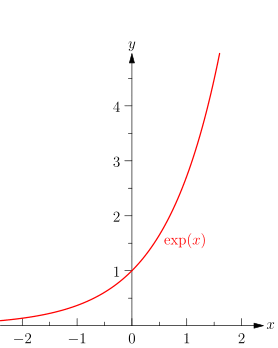
\includegraphics[width=0.5\textwidth, height=\textheight, keepaspectratio]{Mfnf-exp-series-imageonline.co-60931-1.png}
  \end{center}
    
\end{frame}
% slide 2: taylor
\begin{frame}{Taylor Series}
      \begin{center}

    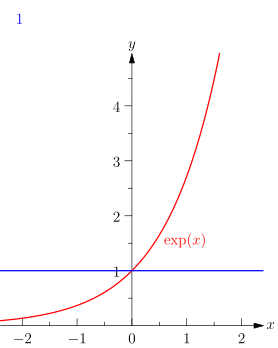
\includegraphics[width=0.5\textwidth, height=\textheight, keepaspectratio]{Mfnf-exp-series-imageonline.co-60931-2.png}
  \end{center}
    
\end{frame}
% slide 2: taylor
\begin{frame}{Taylor Series}
      \begin{center}

    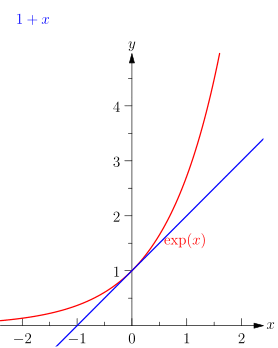
\includegraphics[width=0.5\textwidth, height=\textheight, keepaspectratio]{Mfnf-exp-series-imageonline.co-60931-3.png}
  \end{center}
    
\end{frame}
% slide 2: taylor
\begin{frame}{Taylor Series}
      \begin{center}

    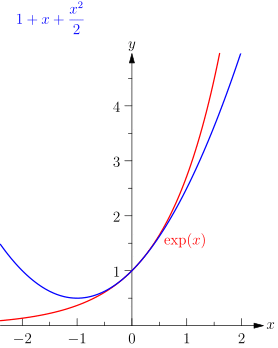
\includegraphics[width=0.5\textwidth, height=\textheight, keepaspectratio]{Mfnf-exp-series-imageonline.co-60931-4.png}
  \end{center}
    
\end{frame}
% slide 2: taylor
\begin{frame}{Taylor Series}
      \begin{center}

    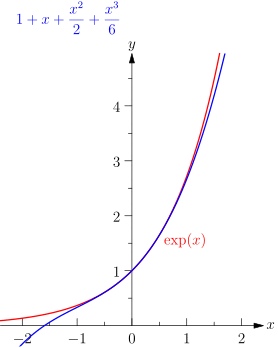
\includegraphics[width=0.5\textwidth, height=\textheight, keepaspectratio]{Mfnf-exp-series-imageonline.co-60931-5.png}
  \end{center}
    
\end{frame}
% slide 2: taylor
\begin{frame}{Taylor Series}
      \begin{center}

    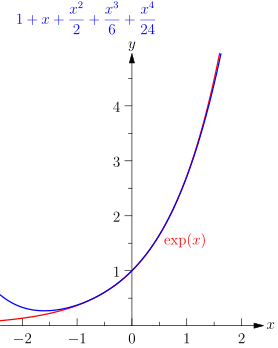
\includegraphics[width=0.5\textwidth, height=\textheight, keepaspectratio]{Mfnf-exp-series-imageonline.co-60931-6.png}
  \end{center}
    
\end{frame}


% slide 2: taylor
\begin{frame}{Taylor Series}
      \begin{center}

    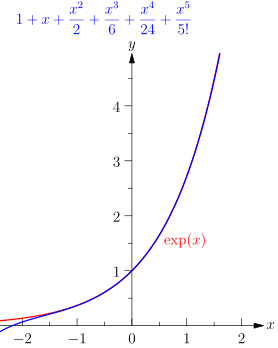
\includegraphics[width=0.5\textwidth, height=\textheight, keepaspectratio]{Mfnf-exp-series-imageonline.co-60931-7.png}
  \end{center}
    
\end{frame}


% slide 2: taylor
\begin{frame}{Taylor Series}
      \begin{center}

    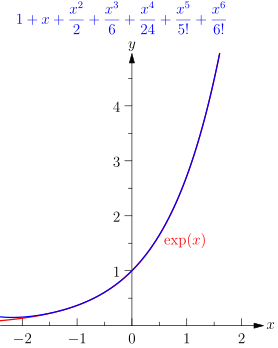
\includegraphics[width=0.5\textwidth, height=\textheight, keepaspectratio]{Mfnf-exp-series-imageonline.co-60931-8.png}
  \end{center}
    
\end{frame}


% slide 2: taylor
\begin{frame}{Taylor Series}
      \begin{center}

    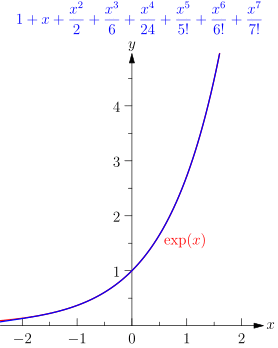
\includegraphics[width=0.5\textwidth, height=\textheight, keepaspectratio]{Mfnf-exp-series-imageonline.co-60931-9.png}
  \end{center}
    
\end{frame}




% slide 3: naxnakan
\begin{frame}{Indefinite Integral}
     So in some sense, if we have the values of the 1st, 2nd, ..., \textit{k}-th order derivatives of a function at some point, we can "reconstruct" the original function (near that point). \pause Can we reconstruct the function if we have \textit{only} the value of $f'(x)$ but at \textit{all} points of some interval?
     \vspace{0.3cm}

\pause
{\color{blue}{Question:}}         Suppose $f'(x)=2x, \: x\in\R$. What does $f(x)$ equal to?

     
     \pause

     {\color{blue}{Answer:}}         $f(x)=x^2$, $f(x)=x^2+1$, etc. -- functions of the form $f(x)=x^2+c$, where $c$ is any constant.
     \pause 
     
       \begin{block}{Definition}
        Let $f:X\to \R$ and $X$ is an interval. The function $F(x)$ is called an \textbf{antiderivative} of $f(x)$ if $F'(x) = f(x)$.
    \end{block}

\end{frame}



% slide 3: naxnakan
\begin{frame}{Indefinite Integral}

    \begin{block}{Properties}
       \begin{enumerate}[<+->]
           \item \[\int af(x) \,dx = a \int  f(x) \,dx\]
           \item \[\int (f(x) + g(x)) \,dx = \int f(x) \,dx + \int g(x) \,dx\]
           \item \[\int f(x)g'(x) \, dx = f(x)g(x) - \int f'(x)g(x) \, dx\]
           
           \pause This can also be written as:
           \[
           \int f \,dg = fg - \int g \,df,
           \]
           where \(\displaystyle \int f \, dg = \int f g' \, dx \).
       \end{enumerate}
    \end{block}

\end{frame}

% slide 3: naxnakan
\begin{frame}{Indefinite Integral}
     \begin{itemize}[<+->]
         \item The antiderivative of any constant $f(x)=a$ is:
         \[\int a \, dx= ax+C\]
         \item The antiderivative of $f(x)=x$ is:
         \[\int x \,dx = \frac{x^2}{2} + C\]
         \item For any constant $n\ne 1$, the derivative of $f(x)=x^n$ is:
         \[\int x^n \,dx = \frac{x^{n+1}}{n+1} + C\]
         \item The antiderivative of $f(x)=\frac{1}{x}$ is:
         \[\int \frac{1}{x} \,dx = \ln|x| + C  \]
     \end{itemize}

\end{frame}


% slide 3: naxnakan
\begin{frame}{Indefinite Integral}
     \begin{itemize}[<+->]
         \item The antiderivative of $f(x)=e^x$ is:
         \[\int e^x \,dx = e^x + C\]
         \item The antiderivative of $f(x)=\cos x$ is:
         \[\int \cos x \,dx = \sin x + C\]
         \item The antiderivative of $f(x)=\sin x$ is:
         \[\int \sin x \,dx = -\cos x  + C\]
         \item The antiderivative of $f(x)=\frac{1}{1+x^2} $ is:
         \[\int \frac{1}{1+x^2} \,dx = \text{arctg}\, x + C  \]
         % \item The antiderivative of $f(x)=\frac{1}{\sqrt{1-x^2}} $ is:
         % \[\int \frac{1}{\sqrt{1-x^2}} \,dx = \arcsin x + C \]
     \end{itemize}

\end{frame}



% slide 4: integral
\begin{frame}{Definite Integral}
Suppose we are given the velocity of a car at each timepoint. How can we calculate the displacement of the car?
\begin{center}
    \includesvg[ width=0.5\textwidth, keepaspectratio]{vt}

\end{center}
\pause Answer: By calculating the area under the curve.


\end{frame}

% slide 4: integral
\begin{frame}{Definite Integral}
Now suppose we have a continuous function $f:[a,b]\to\R$. How can we calculate the area under its graph? \pause By dividing it into tiny rectangles and adding up their areas.

\begin{center}

    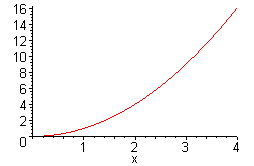
\includegraphics[width=0.35\textwidth, height=\textheight, keepaspectratio]{p1.png}   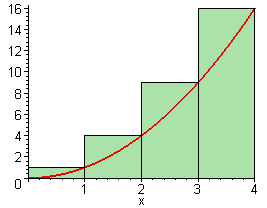
\includegraphics[width=0.33\textwidth, height=\textheight, keepaspectratio]{p2.png}   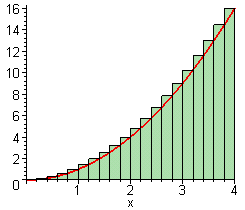
\includegraphics[width=0.3\textwidth, height=\textheight, keepaspectratio]{p3.png}
  \end{center}
  % \pause To do this we need some another kind of integrals.
\end{frame}


% slide 4: integral
\begin{frame}{Definite Integral}
Let $f:[a,b]\to\R$. We divide $[a,b]$ into $n$ subintervals using the points $\{x_0, x_1, \ldots, x_n\}$ which we call a partition of $[a,b]$.\pause
\begin{block}{Definition}
        The \textbf{Riemann sum} of a function $f(x)$ over a partition $\{x_0, x_1, \ldots, x_n\}$ of the interval $[a, b]$ is given by:
        \[
        R_n = \sum_{i=1}^{n} f(c_i) \Delta x_i
        \]
        where $\Delta x_i = x_i - x_{i-1}$ is the width of the $i$-th subinterval, and $c_i$ is any point in the $i$-th subinterval. \pause
         If the limit on the right exists, 
 \[\int_a^b f(x)\, dx = \lim_{n
            \to \infty} \sum_{i=1}^n f(c_i) \,\Delta x_i\]
            is called the \textbf{definite integral} of the function $f(x)$ on $[a,b]$.
            \end{block}
\end{frame}


% slide 4: integral
\begin{frame}{Definite Integral}
 
    The definite integral $\int_a^b f(x) \, dx$ represents the \textbf{signed area} between the graph of $f(x)$ and the $x$-axis over the interval $[a, b]$.

      \begin{center}

    \includesvg[ width=0.8\textwidth, keepaspectratio]{area}
    
  \end{center}

- \color{blue} \href{https://www.sfu.ca/math-coursenotes/Math\%20158\%20Course\%20Notes/sec_defint.html#:~:text=1.4.2\%20Defining\%20the\%20Definite\%20Integral}{Play with Riemann sums!}
\end{frame}



% slide 4: integral
\begin{frame}{Definite Integral}
 How can we calculate the definite integral without limits?\pause
    \begin{block}{Theorem}
        Suppose that $f
(
x
)$
 is continuous on the interval 
$[
a
,
b
]$.
 If 
$F
(
x
)
$ is any antiderivative of 
$f
(
x
)
$,
 then
 \[\int_a^b f(x)\,dx = F(b)-F(a)\]
    \end{block}
\pause
\begin{example}
    \begin{itemize}%[<+->]
        \item
        \[
\int_{0}^{2} x^2 \,dx =\frac{1}{3} \cdot  x^3 \bigg\vert_{0}^{2} = \frac{1}{3} (2^3 - 0^3) =\frac{8}{3}
\]
        \item %Area under $f(x)=x^2$ between $0$ and 2 is:
       \[
\int_{0}^{\pi} \sin x \,dx =  -\cos x \bigg\vert_{0}^{\pi} = -\cos \pi - (-\cos0) = 2
\]

    \end{itemize}
\end{example}
\end{frame}


% slide 4: integral
\begin{frame}{Definite Integral}
    % \begin{block}{Properties}
    \begin{enumerate}[<+->]
        \item \[\int_{a}^{b} f(x) \,dx = -\int_{b}^{a} f(x) \,dx,\qquad \int_{a}^{a} f(x) \,dx = 0
\]
        \item \[\int_{a}^{b} cf(x) \,dx = c \int_{a}^{b} f(x) \,dx
\]
\item \[\int_{a}^{b} (f(x) \pm g(x)) \,dx = \int_{a}^{b} f(x) \,dx \pm \int_{a}^{b} g(x) \,dx
\]
\item \[\int_{a}^{b} f(x) \,dx = \int_{a}^{c} f(x) \,dx + \int_{c}^{b} f(x) \,dx\]

\item \[\int_{a}^{b} f(x) \,dx = \int_{a}^{b} f(y) \,dy\]
i.e. the name of the variable does not matter.
    \end{enumerate}
    
% \end{block}
\end{frame}



% % slide 4: derivative
% \begin{frame}{Derivative}
%       \begin{center}

%     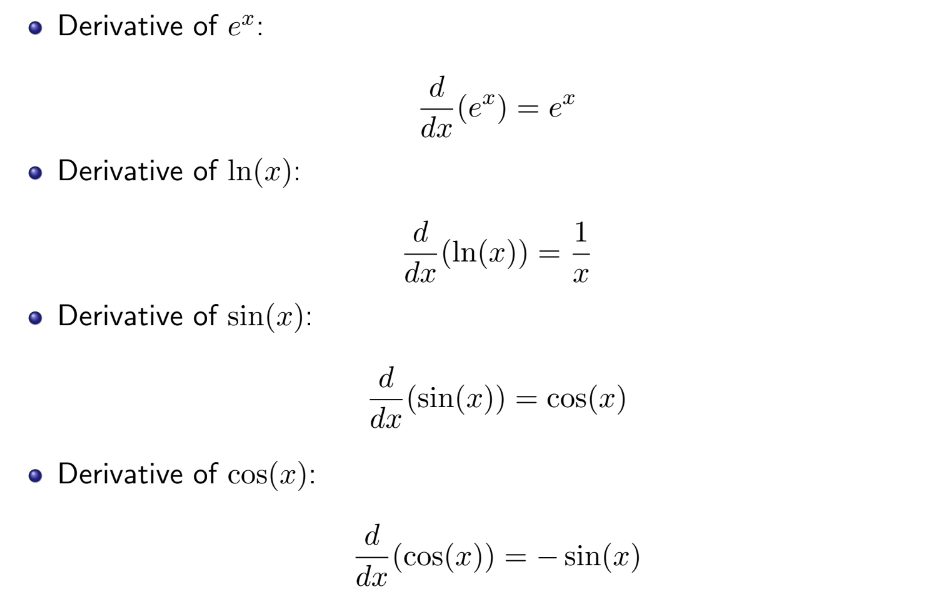
\includegraphics[width=0.9\textwidth, height=\textheight, keepaspectratio]{der2.png}
%   \end{center}
% \end{frame}



% % slide 5: extrema
% \begin{frame}{Extrema of a Function}

% % \begin{center}
% \begin{exampleblock}{Example}
%     Which points are the local extremum points of the following functions? \\ \bigskip
% % \\\includesvg[ width=0.31\textwidth, keepaspectratio]{image-295}\pause 
%  \includesvg[ width=0.31\textwidth, keepaspectratio]{image-296}\pause
%  \includesvg[ width=0.31\textwidth, keepaspectratio]{image-297}\pause
%  \includesvg[ width=0.31\textwidth, keepaspectratio]{image-290}
% \end{exampleblock}
%   % \end{center}
% \pause
% \begin{block}{Theorem}
% If a function \(f\) is continuous on a \textit{closed interval} \([a, b]\), then \(f\) has both a global maximum and a global minimum on \([a, b]\).
    
% \end{block}

  
% \end{frame}


\end{document}
